% arara: pdflatex
% arara: nomencl
% arara: pdflatex
% !TEX TS-program = arara
\documentclass[11pt]{article}
\usepackage{geometry}         
\geometry{letterpaper}    
\usepackage{graphicx}
\usepackage{amssymb}
\usepackage{amsmath}
\usepackage{epstopdf}
\usepackage[]{nomencl}
\usepackage{float} 
\usepackage{enumitem}
\usepackage{lipsum}
\usepackage{setspace}
\makenomenclature
\DeclareGraphicsRule{.tif}{png}{.png}{`convert #1 `dirname #1`/`basename #1 .tif`.png}
\DeclareGraphicsRule{.gif}{png}{.png}{`convert #1 `dirname #1`/`basename #1 .gif`.png}

%% START OF MODIFIABLE CODE

\title{Analysis of Variance in R}
\author{Margaux Winter \\ Miguel de los Reyes \\ North Carolina School of Science and Math}

% LEAVE THIS STUFF ALONE  %%%%%%%%%%%%
\begin{document}
\maketitle
%%%%%%%%%%%%%%%%%%%%%%%%

%  CONTINUING MODIFIABLE STUFF

\section{Introductory Reading}

\nomenclature{Glossary term:}{Definition}

The most common type of linear models are analysis of variance (ANOVA) and linear regression models. R is built to handle linear models, and as such it is easy to work with ANOVA. ANOVA is a statistical method used to compare two or more means. These values can be used to determine whether a significant correlation exists between variables. 

We will be using one-way ANOVA, which compares the means between the groups of interest, and determines whether those means are significantly different from each other. If one-way ANOVA returns a significant result, there are at least two group means that are significantly different from each other. It is important to note that ANOVA is an omnibus test statistic, meaning that although ANOVA tells the user is there is a significant difference in means, it is unable to show which means in particular differ.

ANOVA can only be used with certain types of data configurations. To perform ANOVA, data must have a continuous response variable and at least one categorical factor with two or more levels, in lay terms, ANOVA can only be used with numeric values that can be ordered sequentially, with a certain number of possible responses. (i.e. data comparing object's weights, and each new weight is a level) ANOVA is easier to use if data is from from approximately normally distributed populations with equal variances between factor levels, however, as R is built to work with statistics, ANOVA procedures will generally work without incident unless one or more of the distributions or variances are highly skewed.

A basic understanding of statistics how to use R is recommended before performing ANOVA. The ANOVA user will create and order factors, make box plots, and combine and stack data. 
\cite{cran-r}


The following functions will be useful in using ANOVA.

\begin{enumerate}
\item aov
\item as.factor
\item ls.str
\item data.frame
\item stack
\item TukeyHSD
\item levels
\end{enumerate}


\section{Objectives}

In this assignment, we will use ANOVA to analyze data from ELISA HIV Optical Density Readings. ANOVA identifies the causes of variation, and sorts out the corresponding components of variation with associated degrees of freedom. In this case, we are interested in seeing how HIV Optical Density Readings are related to their lot. The type of ANOVA we are using is one-way between groups, as we are comparing one grouping (the optical density readings) to define the groups (lots). 
\setlist{before=\singlespacing,after=\singlespacing}
\singlespacing
By the end of this lesson, the reader should be able to:
\begin{enumerate}
\item Understand the logic behind one-way analysis of variance.
\item Perform one-way analysis of variance in R for any data. 
\item Appropriately interpret results of analysis of variance tests.
\end{enumerate}

\subsection{ANOVA}

We will look at variances in data using R's ANOVA functions.

\subsection{Visualization}

We will also use our fitted models and our ANOVA data to create box plots and line plots. Much of the information gleaned from ANOVA is presented via numeric such as the sum of square, degrees of freedom, and the mean. ANOVA presents the null hypothesis that there is no difference in means of the treatments, and once this hypothesis is proven incorrect, the question arises of how the treatments differ. The post-hoc test also allows the user to find the differences in means, and specifically categorizes the lower and upper means of the data.

Below is a box plot of the data before running ANOVA or TukeyHSD. Constructing a box plot before analyzing the data may prove helpful in deciding what kind of analysis would be preferable.

\begin{figure}[H] %  the "H" means put it where you put this code....but that doesn't always work!
   \centering
      \caption{Boxplot}
   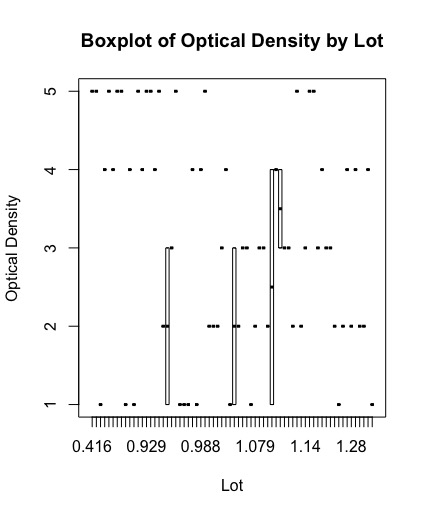
\includegraphics[scale=0.5]{BoxPlotOpticalDensity.jpg} 
   \label{fig:BoxPlotOpticalDensity}
\end{figure}

 

\section{Building the Model}

Looking at the data set of interest for ANOVA, note that that data may be in numeric form. Use the function is.numeric to review the data. If this function prints TRUE, use the function as.factor to change data from numeric to factor. In order to make it easier to manipulate data later on, it is recommended that the factored data is renamed. 
\begin{figure}[H] %  the "H" means put it where you put this code....but that doesn't always work!
   \centering
      \caption{as.factor}
   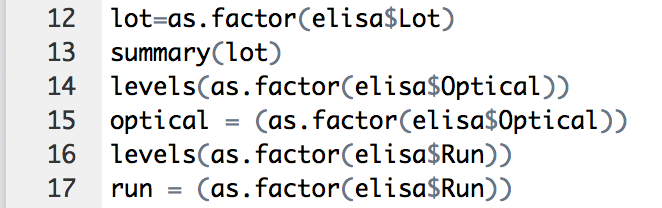
\includegraphics[scale=0.5]{asFactor.png} 
   \label{fig:as.factor}
\end{figure}

Now your factor data type is in non-numerical variables. Each different variable of the factor is called a level. For example, our factor type data for the lots of various ELISA HIV Optical Density Readings has five levels, 1, 2, 3, 4 and 5.

Moving on, we can make a box plot of our data, so that we can visually compare data. Making a summary of this data allows us to look at the residuals and standard error of the plot. As mentioned before, this type of comparison will work better with data that has a relatively normal distribution. 

Factors can also be created within factors. We used our factor Optical to categorize and label by the density. For each level within the main factor, create labels. These labels will designate unordered factors. To make this data easier to read, unordered factors should be ordered. Choose ways to order the data that is relative to the averages in the data. For example, some levels were Low density(below 1) and some were High density,(above 1.5) so we ordered the data starting at 0, then continuing with 1, 1.5, 2. Choose labels that reflect the data, noting that the first label will relate to the lower numbers. Next, classify this newly ordered factor, and now label the data in lay terms. 
\begin{lstlisting}
elisa$Optical.type<-ordered(cut(elisa$Optical, c(0,1,1.5,2), labels = c("Low","Medium","High")))
class(elisa$Optical.type)
elisa$Optical.type
\end{lstlisting}
Note, that if you wish to remove one group of subjects (i.e. Lot 1) R will keep this removed group as a level, possibly skewing your data. Use the function drop levels to remove a selected group as a level. Rename this reconfigured data as to not overwrite your previous data. 

In order to use ANOVA, the data must be in a specific format. To properly configure data, combine the data from the two factors intended to be compared with the function data.frame. Next, stack these combined groups. Finally use this stacked data and the function aov to perform ANOVA. Make a summary of these results.
\begin{lstlisting}
finalelisa <- droplevels(newelisa)
summary(finalelisa$Lot)
Combined_Groups <- data.frame(cbind(lot,optical))
Combined_Groups
Stacked_Groups <- stack(Combined_Groups)
Stacked_Groups
Anova_Results <- aov(values ~ ind, data = Stacked_Groups)
\end{lstlisting}
This method can me used for a simple one-way ANOVA. However some data can compare multiple sets of data against each other. To do this, we can use a post-hoc test. Post-hoc tests compare outcome measurements between multiple groups. With post-hoc analysis the reader can examine differences between pairs of groups after global analysis. Use the function TukeyHSD to perform a pairwise post-hoc analysis on the ANOVA results.
\begin{lstlisting}
summary(Anova_Results)
TukeyHSD(Anova_Results)
summary(TukeyHSD(Anova_Results))
\end{lstlisting}
 \subsection{Programming Hints}
It is recommended to look at data before analysis in order to better understand the levels and attributes of data.
In addition, we recommend the use of summary() and the console to view the attributes of objects.
 

\section{Deliverable}

Using ANOVA, students should be able to take data with sequentially ordered number data, make a box plot, factor the data as unordered and ordered factors, configure the data such that the function aov can be performed, and perform TukeyHSD. Using the box plot, students should be able to identify residuals, coefficients of the linear regression, and residual standard error. 

Using aov, students should be able to identify degrees of freedom, the sum of the squares, the mean of the squares, and the F ratio (the ratio of two mean square values) for their data. 



\section{Teaching Code}

Begin ANOVA by formatting the data in a csv file, then uploading it to RStudio. This script is set up to analyze publicly available data about HIV Optical density readings, but can be adapted for any properly set up data. As the reader works his or her way through the script, be sure to liberally comment the purpose of each command. 

\begin{verbatim}
# Your name here
# Date
# ANOVA - ELISA HIV Optical density readings data

# Clean up and read in data
rm(list=ls())
setwd("C:/Your/Directory")
elisa = read.csv("ELISAHIV.csv")

# Create levels for lot, optical, and run
# Make sure to view/check your data
levels(as.factor(elisa$Lot))
lot=as.factor(elisa$Lot)
# etc.


# Create a boxplot showing optical density by lot
# Make sure to label your axes!
boxplot(..., ...)


# Perform a linear regression of optical density by lot
summary(lm(..., data=elisa))

# Create an ordered factor using Optical.type and verify its type
elisa$Optical.type<-ordered(...)
class(elisa$Optical.type)

# Remove 1 as a possible level
# Note: even if you eliminate a group of subjects (ex. 1),
# because it's a factor, R keeps 1 as a possible level for lot

# Use droplevels() to remove 1

# Create stacked results to run aov()

# Run TukeyHSD on the ANOVA results

\end{verbatim}

\section{Example Student Code}
\begin{verbatim}
# KEY
# ANOVA - ELISA HIV Optical density readings data

# Clean up and read in data
rm(list=ls())
setwd("C:/Example/Code")
elisa = read.csv("ELISAHIV.csv")

# Look at variables and create levels
ls.str(elisa)
levels(as.factor(elisa$Lot))
lot=as.factor(elisa$Lot)
summary(lot)
levels(as.factor(elisa$Optical))
optical = (as.factor(elisa$Optical))
levels(as.factor(elisa$Run))
run = (as.factor(elisa$Run))

# Create a boxplot
boxplot(elisa$Lot~elisa$Optical, xlab="Lot", ylab="Optical Density", 
    main="Boxplot of Optical Density by Lot")
summary(lm(elisa$Optical~elisa$Lot, data=elisa))

# Perform regression
summary(optical)
elisa$Optical.type<-ordered(cut(elisa$Optical, c(0,1,1.5,2),
    labels=c("Low","Medium","High")))
class(elisa$Optical.type)
elisa$Optical.type

# Remove 1 as a level
# We've verified that optical is an ordered factor
# Note: even if you eliminate a group of subjects (ex. 1),
# because it's a factor, R keeps 1 as a possible level for lot
newelisa <- elisa[1:2,]
summary(newelisa$Lot)
# We remove 1 as a possible level using droplevels()
finalelisa <-droplevels(newelisa)

# We create stacked results to run aov()
summary(finalelisa$Lot)
Combined_Groups <- data.frame(cbind(lot,optical))
Combined_Groups
Stacked_Groups <- stack(Combined_Groups)
Stacked_Groups
Anova_Results <- aov(values ~ ind, data = Stacked_Groups)
summary(Anova_Results)

# We also run TukeyHSD on the ANOVA results
TukeyHSD(Anova_Results)
summary(TukeyHSD(Anova_Results))
\end{verbatim}


\section{Further Readings}

\begin{enumerate}
\item Seefeld, Kim and Linder, Ernst. \emph{Statistics Using R
with Biological Examples}, University of New Hampshire, Durham, NH
Department of Mathematics and Statistics(2007)

\item Julian J. Faraway. \emph{Practical Regression and Anova using R}, University of Michigan, (2002)
\end{enumerate}

\begin{thebibliography}{99}

\bibitem{cran-r}
Seefeld, Kim and Linder, Ernst. \emph{Statistics Using R
with Biological Examples}, University of New Hampshire, Durham, NH
Department of Mathematics and Statistics(2007)

\bibitem{data}
National Institute of Standards and Technology, Statistical Engineering Division, Education/Training. (2003). ELISA HIV Optical Density Readings. Retrieved from http://www.itl.nist.gov/div898/education/anova/elisa.dat

\bibitem{TukeyHSD}
ETH Zuric Department of Mathematics. (n.d.). Compute Tukey Honest Significant Differences. Retrieved from https://stat.ethz.ch/R-manual/R-devel/library/stats/html/TukeyHSD.html

 
\end{thebibliography}

\printnomenclature
\end{document}  
